% !TEX program = lualatex
\documentclass[12pt,a4paper]{article}
\usepackage{fontspec}
\setmonofont{Latin Modern Mono}
\usepackage{xcolor}
\usepackage{listings}
\usepackage{geometry}
\usepackage{fancyhdr}
\usepackage{hyperref}
\usepackage{graphicx}
\geometry{margin=1in}
\usepackage{multicol}

% -------------------------------
% SOLUTION TOGGLE
% -------------------------------
\newif\ifshowsolutions
% \showsolutionstrue 
\showsolutionsfalse

% -------------------------------
% Header and Footer Configuration
% -------------------------------
\pagestyle{fancy}
\fancyhf{}
\lhead{Lab Final}
\rhead{CSE 4308: DBMS Lab}
\cfoot{\thepage}
\setlength{\headwidth}{\textwidth}

% -------------------------------
% Code Listing Style
% -------------------------------
\definecolor{codegreen}{rgb}{0,0.6,0}
\definecolor{codegray}{rgb}{0.5,0.5,0.5}
\definecolor{codepurple}{rgb}{0.58,0,0.82}
\definecolor{backcolour}{rgb}{0.95,0.95,0.92}

\lstdefinestyle{mystyle}{
    backgroundcolor=\color{backcolour},
    commentstyle=\color{codegreen},
    keywordstyle=\color{magenta},
    numberstyle=\tiny\color{codegray},
    stringstyle=\color{codepurple},
    basicstyle=\ttfamily\footnotesize,
    breaklines=true,
    captionpos=b,
    keepspaces=true,
    numbers = none,
    numbersep=5pt,
    tabsize=2,
    frame=single,
    columns=fullflexible,
    showspaces=false,
    showstringspaces=false,
    showtabs=false
}

\lstset{style=mystyle}

% Images: found next to this file (local compile_labs.sh) or via the
% lab folder when compiled from the project root (Overleaf).
\graphicspath{{lab_14_final/}}

\begin{document}

% --------------------------------------------------------------
% TITLE PAGE
% --------------------------------------------------------------
\begin{titlepage}
    \centering
    \vspace*{2\baselineskip}

    \rule{14cm}{2pt}\vspace*{-0.8\baselineskip}\vspace*{1.5pt}
    \rule{14cm}{0.5pt}\vspace{2\baselineskip}

    {\Huge\bfseries\scshape Lab Final\par}
    \vspace{3mm}
    {\Large }
    \vspace{3mm}

    \rule{14cm}{0.5pt}\vspace*{-0.7\baselineskip}\vspace{2.5pt}
    \rule{14cm}{2pt}

    \vspace{2\baselineskip}

    {\Large\bfseries CSE 4308\par}
    \vspace{1\baselineskip}
    {\large DATABASE MANAGEMENT SYSTEMS LAB\par}

    \vfill
    {\normalsize Prepared by:\\ Samnun Azfar, Jr. Lecturer, CSE\\ Samia Nawsheen, Jr. Lecturer, CSE\par}
    {\normalsize Academic Year: AY25-26\par}
\end{titlepage}

\newpage
\newpage

% ==============================================================
\section{Lab Final}
\begin{enumerate}
% % ==============================================================
% \item Show all rentals that were made on '2005-05-25'. Display rental id and rental date.

% \ifshowsolutions
% \begin{lstlisting}[language=SQL]
% SELECT rental_id, rental_date
% FROM rental
% WHERE rental_date::date = '2005-05-25';
% \end{lstlisting}
% \fi
% ==============================================================
\item Rank films using a weighted value calculation: (rental\_rate × 0.5) + (length × 0.1) + (replacement\_cost × 0.2). Based on the value, list only the top 3 films with their title, release year, and calculated score.
\ifshowsolutions
\begin{lstlisting}[language=SQL]
SELECT 
    title, 
    release_year, 
    (rental_rate * 0.5) + (length * 0.1) + (replacement_cost * 0.2) AS value_score
FROM film
ORDER BY value_score DESC
LIMIT 3;
\end{lstlisting}
\fi

% ==============================================================
\item Find the top 5 customers who have spent the highest total amount. Show customer ID, first name, last name, and total amount spent.

\ifshowsolutions
\begin{lstlisting}[language=SQL]
SELECT c.customer_id, c.first_name, c.last_name,
       SUM(p.amount) AS total_spent
FROM customer c
JOIN payment p ON p.customer_id = c.customer_id
GROUP BY c.customer_id, c.first_name, c.last_name
ORDER BY total_spent DESC
LIMIT 5;
\end{lstlisting}
\fi

% ==============================================================
\item List all film titles consisting of more than one word that have been rented by customers from at least two different cities. Also list the total number of unique customers who rented each of those films, sorted by the customer count in descending order.

\ifshowsolutions
\begin{lstlisting}[language=SQL]
SELECT 
    f.title,
    COUNT(DISTINCT c.customer_id) AS customer_count
FROM film f
JOIN inventory i ON f.film_id = i.film_id
JOIN rental r ON i.inventory_id = r.inventory_id
JOIN customer c ON r.customer_id = c.customer_id
JOIN address a ON c.address_id = a.address_id
JOIN city ci ON a.city_id = ci.city_id
WHERE f.title LIKE '% %'
GROUP BY f.film_id, f.title
HAVING COUNT(DISTINCT ci.city_id) >= 2
ORDER BY customer_count DESC;
\end{lstlisting}
\fi


% ==============================================================

% \item Write an anonymous block that prints how many rentals involve films whose rental rate is greater than 4.

% \ifshowsolutions
% \begin{lstlisting}[language=SQL]
% DO $$
% DECLARE
%     v_count INT;
% BEGIN
%     SELECT COUNT(*)
%     INTO v_count
%     FROM rental r
%     JOIN inventory i ON r.inventory_id = i.inventory_id
%     JOIN film f ON f.film_id = i.film_id
%     WHERE f.rental_rate > 4;

%     RAISE NOTICE 'Total expensive rentals: %', v_count;
% END $$;
% \end{lstlisting}
% \fi
% ==============================================================
\item List the country having the most number of cities without any registered customers.
\ifshowsolutions
\begin{lstlisting}[language=SQL]
SELECT 
    co.country, 
    COUNT(ci.city_id) AS empty_cities_count
FROM country co
JOIN city ci ON co.country_id = ci.country_id
LEFT JOIN address a ON ci.city_id = a.city_id
LEFT JOIN customer c ON a.address_id = c.address_id
WHERE c.customer_id IS NULL
GROUP BY co.country_id, co.country
ORDER BY empty_cities_count DESC
LIMIT 1;
\end{lstlisting}
\fi
% ==============================================================
% \item Show each category name along with the total number of rentals for films in that category. Order by total rentals descending.

% \ifshowsolutions
% \begin{lstlisting}[language=SQL]
% SELECT c.name,
%        COUNT(r.rental_id) AS total_rentals
% FROM category c
% JOIN film_category fc ON fc.category_id = c.category_id
% JOIN inventory i ON i.film_id = fc.film_id
% JOIN rental r ON r.inventory_id = i.inventory_id
% GROUP BY c.name
% ORDER BY total_rentals DESC;
% \end{lstlisting}
% \fi
% ==============================================================
\item Write a procedure named \texttt{update\_customer\_email} that accepts a customer ID and a new email string. Update the targeted customer's email address and refresh their \texttt{last\_update} timestamp.

\ifshowsolutions
\begin{lstlisting}[language=SQL]
CREATE OR REPLACE PROCEDURE update_customer_email(
    p_customer_id INT,
    p_new_email VARCHAR
)
LANGUAGE plpgsql
AS $$
BEGIN
    UPDATE customer
    SET email = p_new_email,
        last_update = CURRENT_TIMESTAMP
    WHERE customer_id = p_customer_id;
END;
$$;

DO $$
BEGIN
    CALL update_customer_email(1, 'new.email@example.com');
END;
$$;
\end{lstlisting}
\fi

% ==============================================================
% \item Write an anonymous block to print all rental IDs for customer ID = 1.

% \ifshowsolutions
% \begin{lstlisting}[language=SQL]
% DO $$
% DECLARE
%     rec RECORD;
% BEGIN
%     FOR rec IN
%         SELECT rental_id
%         FROM rental
%         WHERE customer_id = 1
%     LOOP
%         RAISE NOTICE 'Rental ID: %', rec.rental_id;
%     END LOOP;
% END $$;
% \end{lstlisting}
% \fi
\item Write an anonymous block that checks whether a given customer ID currently has any active rentals. Print a notice stating either:
(i) "Customer has active rentals", or
(ii) "Customer has no active rentals".

\ifshowsolutions
\begin{lstlisting}[language=SQL]
DO $$
DECLARE
    v_customer_id INT := 155;
    v_count INT;
BEGIN
    SELECT COUNT(*)
    INTO v_count
    FROM rental
    WHERE customer_id = v_customer_id
      AND return_date IS NULL;

    IF v_count > 0 THEN
        RAISE NOTICE 'Customer % has active rentals', v_customer_id;
    ELSE
        RAISE NOTICE 'Customer % has no active rentals', v_customer_id;
    END IF;
END $$;
\end{lstlisting}
\fi
% ==============================================================
\item Write an anonymous block to show all films with a replacement cost greater than 28.00.
\ifshowsolutions
\begin{lstlisting}[language=SQL]
DO $$
DECLARE
    film_record RECORD;
BEGIN
    FOR film_record IN 
        SELECT title, replacement_cost 
        FROM film 
        WHERE replacement_cost > 28.00
    LOOP
        RAISE NOTICE 'Film: %, Cost: $%', film_record.title, film_record.replacement_cost;
    END LOOP;
END;
$$ LANGUAGE plpgsql;
\end{lstlisting}
\fi
% ==============================================================
\item Write an anonymous block that defines a customer ID and a start date. Calculate and print their total spend from that start date up to the current date.

\ifshowsolutions
\begin{lstlisting}[language=SQL]
DO $$
DECLARE
    v_customer_id INT := 1;
    v_start_date TIMESTAMP := '2005-05-01 00:00:00';
    v_total_spent DECIMAL(10,2);
BEGIN
    -- Calculate total spent from start date to current date
    SELECT COALESCE(SUM(amount), 0.00)
    INTO v_total_spent
    FROM payment
    WHERE customer_id = v_customer_id
      AND payment_date >= v_start_date
      AND payment_date <= CURRENT_TIMESTAMP;

    -- Display the captured results
    RAISE NOTICE 'Total Spent: $%', v_total_spent;
END;
$$;
\end{lstlisting}
\fi
% ==============================================================
\item Create a function that prints customers who did not rent any film in the last N days, taking the number of days as an input parameter.
\ifshowsolutions
\begin{lstlisting}[language=SQL]
CREATE OR REPLACE FUNCTION print_inactive_customers(p_days INT)
RETURNS VOID
LANGUAGE plpgsql
AS $$
DECLARE
    rec RECORD;
BEGIN
    FOR rec IN
        SELECT c.customer_id, c.first_name, c.last_name
        FROM customer c
        WHERE NOT EXISTS (
            SELECT *
            FROM rental r
            WHERE r.customer_id = c.customer_id
            AND r.rental_date >= NOW() - (p_days * INTERVAL '1 day')
        )
    LOOP
        RAISE NOTICE 'Inactive: % %', rec.first_name, rec.last_name;
    END LOOP;
END;
$$;
SELECT print_inactive_customers(30);
\end{lstlisting}
\fi

% ==============================================================
\item Calculate each customer's percentage of their store's total revenue. Show their name and store ID.

\ifshowsolutions
\begin{lstlisting}[language=SQL]
WITH CustomerRevenue AS (
    SELECT 
        c.store_id, 
        c.first_name, 
        c.last_name, 
        SUM(p.amount) AS spent
    FROM customer c
    JOIN payment p ON c.customer_id = p.customer_id
    GROUP BY c.store_id, c.first_name, c.last_name
)
SELECT 
    cr.store_id, 
    cr.first_name, 
    cr.last_name, 
    ROUND((cr.spent / (SELECT SUM(spent) FROM CustomerRevenue WHERE store_id = cr.store_id)) * 100, 2) AS contribution_percentage
FROM CustomerRevenue cr
ORDER BY cr.store_id, contribution_percentage DESC;
\end{lstlisting}
\fi


\end{enumerate}
\newpage
\section{ER Diagram}
\begin{figure}[htbp]
    \centering
    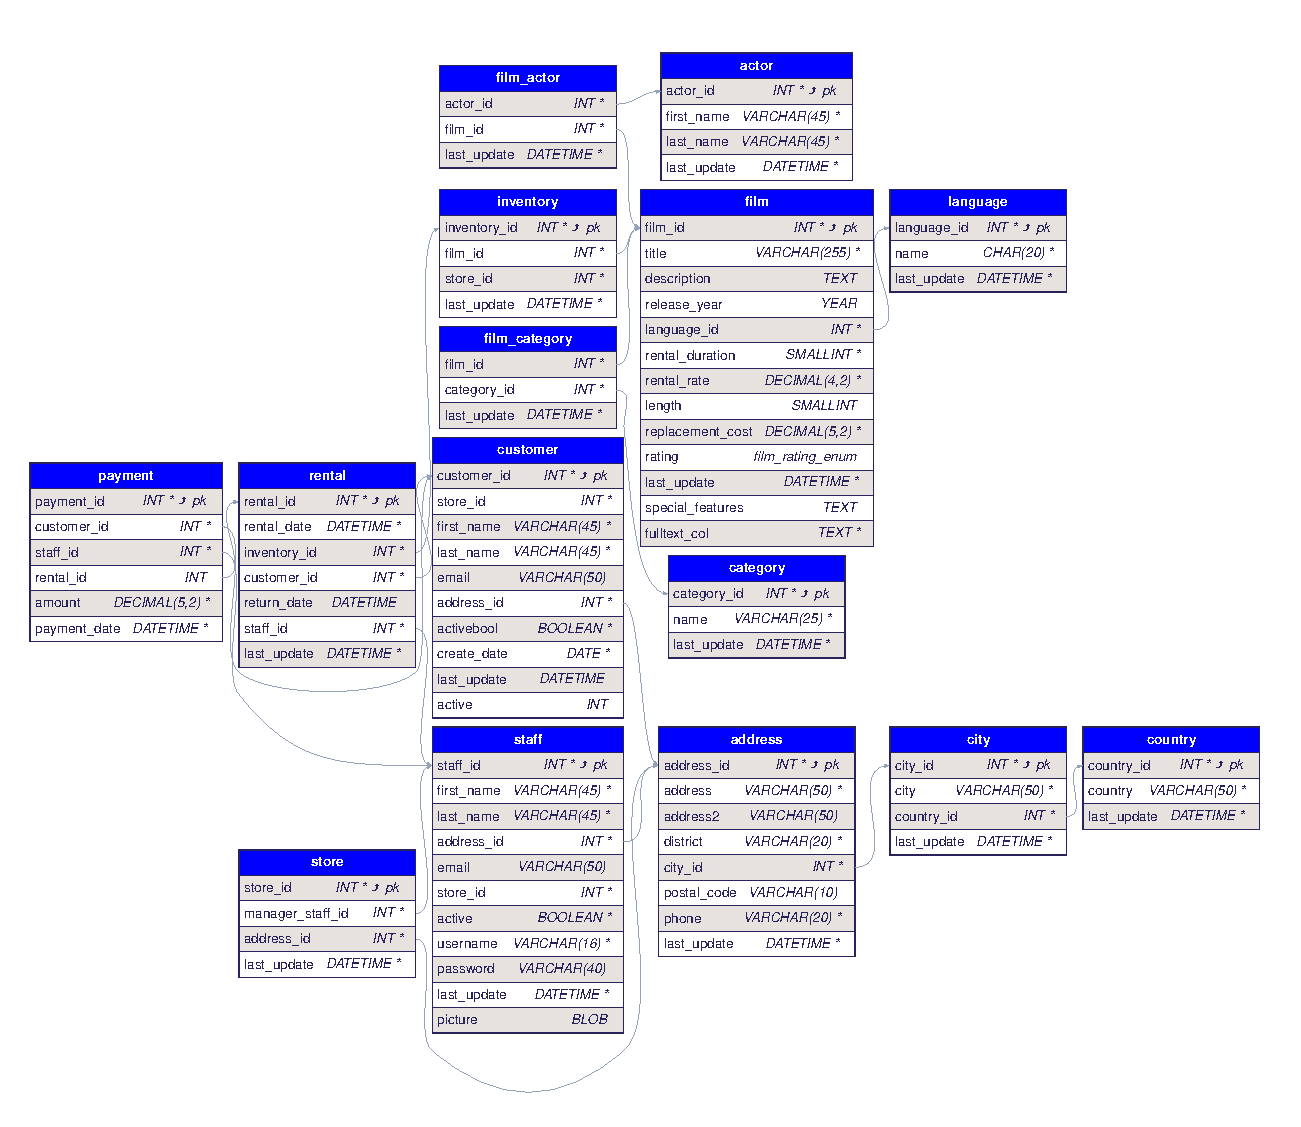
\includegraphics[width=\textheight, height=\textwidth, keepaspectratio, angle=90]{lab_14_schema_cropped.pdf}
\end{figure}
\end{document}